%% This is the ctufit-thesis example file. It is used to produce theses
%% for submission to Czech Technical University, Faculty of Information Technology.
%%
%% Get the newest version from
%% https://gitlab.fit.cvut.cz/theses-templates/FITthesis-LaTeX
%%
%%
%% Copyright 2021, Eliska Sestakova and Ondrej Guth
%%
%% This work may be distributed and/or modified under the
%% conditions of the LaTeX Project Public Licenese, either version 1.3
%% of this license or (at your option) any later version.
%% The latest version of this license is in
%%  https://www.latex-project.org/lppl.txt
%% and version 1.3 or later is part of all distributions of LaTeX
%% version 2005/12/01 or later.
%%
%% This work has the LPPL maintenance status `maintained'.
%%
%% The current maintainer of this work is Ondrej Guth.
%% Contact ondrej.guth@fit.cvut.cz for bug reports.
%% Alternatively, submit bug reports into the tracker at
%% https://gitlab.fit.cvut.cz/theses-templates/FITthesis-LaTeX/issues
%%
%%

%%%%%%%%%%%%%%%%%%%%%%%%%%%%%%%%%%%%%%%%%
% CLASS OPTIONS
% language: czech/english/slovak
% thesis type: bachelor/master/dissertation
% colour: bw for black&white OR no option for default colour scheme
%%%%%%%%%%%%%%%%%%%%%%%%%%%%%%%%%%%%%%%%%
\documentclass[slovak,master,unicode,bw]{ctufit-thesis}

%%%%%%%%%%%%%%%%%%%%%%%%%%%%%%%%%%
% FILL IN THIS INFORMATION
%%%%%%%%%%%%%%%%%%%%%%%%%%%%%%%%%%
\ctufittitle{Webové rozhranie pre spracovanie SPAMM tagovaných dát z magnetickej rezonancie} % replace with the title of your thesis
\ctufitauthorfull{Bc. Tomáš Taro} % replace with your full name (first name(s) and then family name(s) / surname(s)) including academic degrees
\ctufitauthorsurnames{Taro} % replace with your surname(s) / family name(s)
\ctufitauthorgivennames{Tomáš} % replace with your first name(s) / given name(s)
\ctufitsupervisor{Ing. Petr Pauš, Ph.D.} % replace with name of your supervisor/advisor (include academic degrees)
\ctufitdepartment{Katedra softwarového inženýrství} % replace with the department of your defence
\ctufityear{2023} % replace with the year of your defence
\ctufitdeclarationplace{Prahe} % replace with the place where you sign the declaration
\ctufitdeclarationdate{\today} % replace with the date of signature of the declaration
\ctufitabstractCZE{Fill in abstract of this thesis in Czech language. Class aptent taciti sociosqu ad litora torquent per conubia nostra, per inceptos hymenaeos. Cras pede libero, dapibus nec, pretium sit amet, tempor quis. Sed vel lectus. Donec odio tempus molestie, porttitor ut, iaculis quis, sem. Suspendisse sagittis ultrices augue.}
\ctufitabstractENG{Fill in abstract of this thesis in English language. Class aptent taciti sociosqu ad litora torquent per conubia nostra, per inceptos hymenaeos. Cras pede libero, dapibus nec, pretium sit amet, tempor quis. Sed vel lectus. Donec odio tempus molestie, porttitor ut, iaculis quis, sem. Suspendisse sagittis ultrices augue.}
\ctufitkeywordsCZE{enter, commma, separated, list, of, keywords, in, CZECH}
\ctufitkeywordsENG{enter, commma, separated, list, of, keywords, in, ENGLISH}
%%%%%%%%%%%%%%%%%%%%%%%%%%%%%%%%%%
% END FILL IN
%%%%%%%%%%%%%%%%%%%%%%%%%%%%%%%%%%

%%%%%%%%%%%%%%%%%%%%%%%%%%%%%%%%%%
% CUSTOMIZATION of this template
% Skip this part or alter it if you know what you are doing.
%%%%%%%%%%%%%%%%%%%%%%%%%%%%%%%%%%

\RequirePackage{iftex}[2020/03/06]
\iftutex % XeLaTeX and LuaLaTeX
    \RequirePackage{ellipsis}[2020/05/22] %ellipsis workaround for XeLaTeX
\else
    \RequirePackage[utf8]{inputenc}[2018/08/11] %this file encoding
    \RequirePackage{lmodern}[2009/10/30] % vector flavor of Computer Modern font
\fi

% hyperlinks
\RequirePackage[pdfpagelayout=TwoPageRight,colorlinks=false,allcolors=decoration,pdfborder={0 0 0.1}]{hyperref}[2020-05-15]

% uncomment the following to hide all hyperlinks 
% \RequirePackage[pdfpagelayout=TwoPageRight,hidelinks]{hyperref}[2020-05-15]

\RequirePackage{pdfpages}[2020/01/28]

\setcounter{secnumdepth}{4} % numbering sections; 4: subsubsection



%%%%%%%%%%%%%%%%%%%%%%%%%%%%%%%%%%
% CUSTOMIZATION of this template END
%%%%%%%%%%%%%%%%%%%%%%%%%%%%%%%%%%


%%%%%%%%%%%%%%%%%%%%%%
% DEMO CONTENTS SETTINGS
% You may choose to modify this part.
%%%%%%%%%%%%%%%%%%%%%%
\usepackage{dirtree}
\usepackage{lipsum,tikz}
\usepackage{csquotes}
\usepackage[style=iso-numeric]{biblatex}
\addbibresource{text/bib-database.bib}
\usepackage{listings} % typesetting of sources
\usepackage[colorinlistoftodos]{todonotes}
\usepackage{float}
% \usepackage{xevlna}
\setlength{\marginparwidth}{2.5cm}
% \usepackage{minted} % typesetting of sources

%theorems, definitions, etc.
\theoremstyle{plain}
\newtheorem{theorem}{Věta}
\newtheorem{lemma}[theorem]{Tvrzení}
\newtheorem{corollary}[theorem]{Důsledek}
\newtheorem{proposition}[theorem]{Návrh}
\newtheorem{definition}[theorem]{Definícia}
\theoremstyle{definition}
\newtheorem{example}[theorem]{Příklad}
\theoremstyle{remark}
\newtheorem{note}[theorem]{Poznámka}
\newtheorem*{note*}{Poznámka}
\newtheorem{remark}[theorem]{Pozorování}
\newtheorem*{remark*}{Pozorování}
\numberwithin{theorem}{chapter}
%theorems, definitions, etc. END
%%%%%%%%%%%%%%%%%%%%%%
% DEMO CONTENTS SETTINGS END
%%%%%%%%%%%%%%%%%%%%%%

\begin{document} 
\frontmatter\frontmatterinit % do not remove these two commands

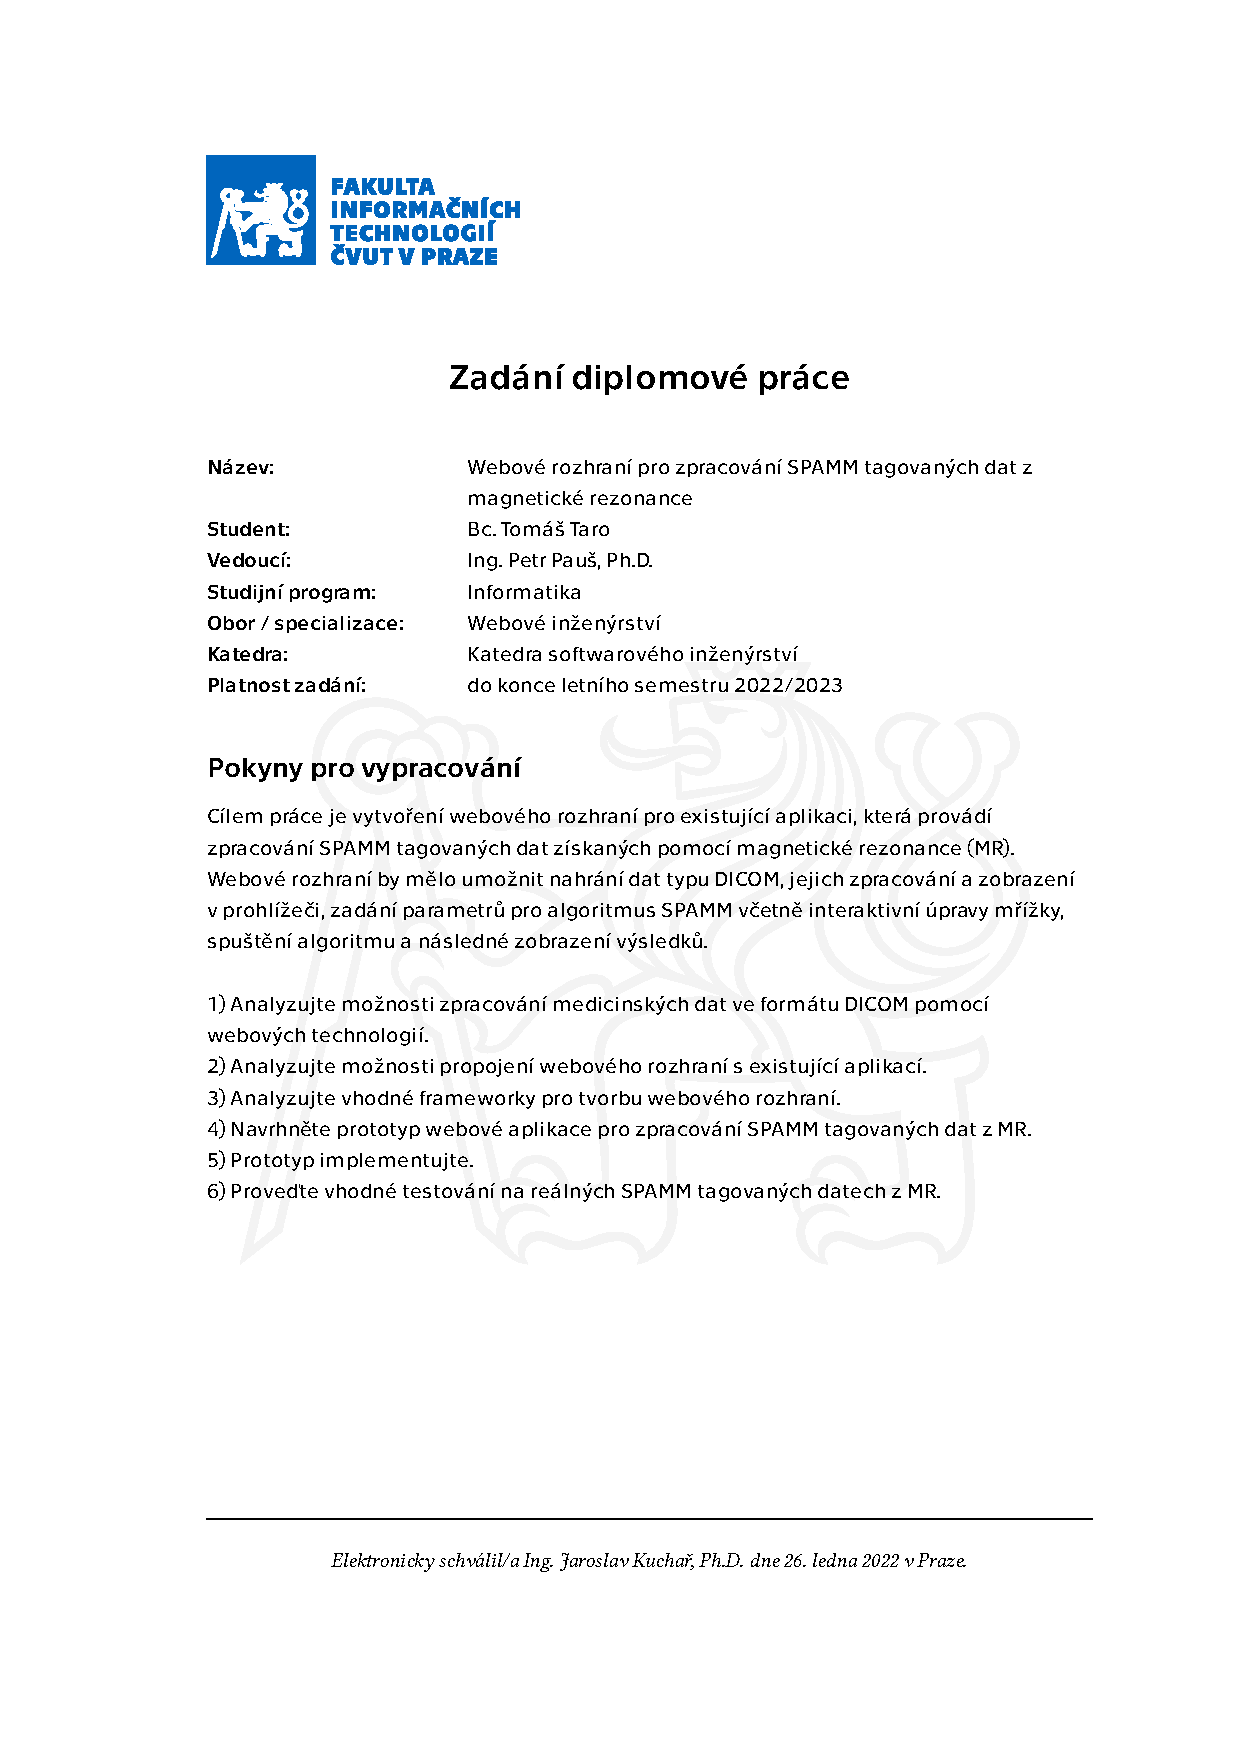
\includepdf[pages={1-}]{media/zadanie_DP_Tomáš_Taro.pdf} % replace that file with your thesis assignment provided by study office

\thispagestyle{empty}\cleardoublepage\maketitle % do not remove these three commands

\imprintpage % do not remove this command

\tableofcontents % do not remove this command
%%%%%%%%%%%%%%%%%%%%%%
% list of other contents: figures, tables, code listings, algorithms, etc.
% add/remove commands accordingly
%%%%%%%%%%%%%%%%%%%%%%
\listoffigures % list of figures
\begingroup
\let\clearpage\relax
\listoftables % list of tables
\lstlistoflistings % list of source code listings generated by the listings package
% \listoflistings % list of source code listings generated by the minted package
\endgroup
%%%%%%%%%%%%%%%%%%%%%%
% list of other contents END
%%%%%%%%%%%%%%%%%%%%%%

%%%%%%%%%%%%%%%%%%%
% ACKNOWLEDGMENT
% FILL IN / MODIFY
% This is a place to thank people for helping you. It is common to thank your supervisor.
%%%%%%%%%%%%%%%%%%%
\begin{acknowledgmentpage}
	Chtěl bych poděkovat především sit amet, consectetuer adipiscing elit. Curabitur sagittis hendrerit ante. Class aptent taciti sociosqu ad litora torquent per conubia nostra, per inceptos hymenaeos. Cras pede libero, dapibus nec, pretium sit amet, tempor quis. Sed vel lectus. Donec odio tempus molestie, porttitor ut, iaculis quis, sem. Suspendisse sagittis ultrices augue.
\end{acknowledgmentpage} 
%%%%%%%%%%%%%%%%%%%
% ACKNOWLEDGMENT END
%%%%%%%%%%%%%%%%%%%


%%%%%%%%%%%%%%%%%%%
% DECLARATION
% FILL IN / MODIFY
%%%%%%%%%%%%%%%%%%%
% INSTRUCTIONS
% ENG: choose one of approved texts of the declaration. DO NOT CREATE YOUR OWN. Find the approved texts at https://courses.fit.cvut.cz/SFE/download/index.html#_documents (document Declaration for FT in English)
% CZE/SLO: Vyberte jedno z fakultou schvalenych prohlaseni. NEVKLADEJTE VLASTNI TEXT. Schvalena prohlaseni najdete zde: https://courses.fit.cvut.cz/SZZ/dokumenty/index.html#_dokumenty (prohlášení do ZP)
\begin{declarationpage}
FILL IN ACCORDING TO THE INSTRUCTIONS. VYPLŇTE V SOULADU S POKYNY. Lorem ipsum dolor sit amet, consectetuer adipiscing elit. Curabitur sagittis hendrerit ante. Class aptent taciti sociosqu ad litora torquent per conubia nostra, per inceptos hymenaeos. Cras pede libero, dapibus nec, pretium sit amet, tempor quis. Sed vel lectus. Donec odio tempus molestie, porttitor ut, iaculis quis, sem. Suspendisse sagittis ultrices augue. Donec ipsum massa, ullamcorper in, auctor et, scelerisque sed, est. In sem justo, commodo ut, suscipit at, pharetra vitae, orci. Pellentesque pretium lectus id turpis.

Lorem ipsum dolor sit amet, consectetuer adipiscing elit. Curabitur sagittis hendrerit ante. Class aptent taciti sociosqu ad litora torquent per conubia nostra, per inceptos hymenaeos. Cras pede libero, dapibus nec, pretium sit amet, tempor quis. Sed vel lectus. Donec odio tempus molestie, porttitor ut, iaculis quis, sem. Suspendisse sagittis ultrices augue. Donec ipsum massa, ullamcorper in, auctor et, scelerisque sed, est. In sem justo, commodo ut, suscipit at, pharetra vitae, orci. Pellentesque pretium lectus id turpis.
\end{declarationpage}
%%%%%%%%%%%%%%%%%%%
% DECLARATION END
%%%%%%%%%%%%%%%%%%%

\printabstractpage % do not remove this command

%%%%%%%%%%%%%%%%%%%
% SUMMARY
% FILL IN / MODIFY
% OR REMOVE ENTIRELY (upon agreement with your supervisor)
% (appropriate to remove in most theses)
%%%%%%%%%%%%%%%%%%%
% \begin{summarypage}
% \section*{Summary section}

% \lipsum[1][1-8]

% \section*{Summary section}

% \lipsum[2][1-6]

% \section*{Summary section}

% \lipsum[3]

% \section*{Summary section}

% \lipsum[2]

% \section*{Summary section}

% \lipsum[1][1-8] Lorem lorem lorem.
% \end{summarypage}
%%%%%%%%%%%%%%%%%%%
% SUMMARY END
%%%%%%%%%%%%%%%%%%%

%%%%%%%%%%%%%%%%%%%
% ABBREVIATIONS
% FILL IN / MODIFY
% OR REMOVE ENTIRELY
% List the abbreviations in lexicography order.
%%%%%%%%%%%%%%%%%%%
\chapter{Zoznam skratiek}
	
\begin{tabular}{rl}
CT & Počítačová tomografia\\
MR & Magnetická rezonancia\\
SPAMM & Spatial Modulation of Magnetization
\end{tabular}
%%%%%%%%%%%%%%%%%%%
% ABBREVIATIONS END
%%%%%%%%%%%%%%%%%%%

\mainmatter\mainmatterinit % do not remove these two commands

%%%%%%%%%%%%%%%%%%%
% THE THESIS
% MODIFY ANYTHING BELOW THIS LINE
%%%%%%%%%%%%%%%%%%%

% % Do not forget to include Introduction
%---------------------------------------------------------------
% \chapter{Introduction}
% uncomment the following line to create an unnumbered chapter
\chapter*{Introduction}\addcontentsline{toc}{chapter}{Introduction}\markboth{Introduction}{Introduction}
%---------------------------------------------------------------
\setcounter{page}{1}

% The following environment can be used as a mini-introduction for a chapter. Use that any way it pleases you (or comment it out). It can contain, for instance, a summary of the chapter. Or, there can be a quotation.
\begin{chapterabstract}
	\lipsum[1]
\end{chapterabstract}

\lipsum[2][1-4]{} [1]

\lipsum[4]

%---------------------------------------------------------------
\section{Ut enim ad minim veniam}
%---------------------------------------------------------------

\lipsum[6-7]

\begin{figure}
\centering
%\includegraphics[scale=0.4]{pic/index}
\resizebox{\textwidth}{!}{
\begin{tikzpicture}[level/.style={sibling distance=60mm/#1}]
\node [circle,draw] (z){$n$}
  child {node [circle,draw] (a) {$\frac{n}{2}$}
    child {node [circle,draw] (b) {$\frac{n}{2^2}$}
      child {node {$\vdots$}
        child {node [circle,draw] (d) {$\frac{n}{2^k}$}}
        child {node [circle,draw] (e) {$\frac{n}{2^k}$}}
      } 
      child {node {$\vdots$}}
    }
    child {node [circle,draw] (g) {$\frac{n}{2^2}$}
      child {node {$\vdots$}}
      child {node {$\vdots$}}
    }
  }
  child {node [circle,draw] (j) {$\frac{n}{2}$}
    child {node [circle,draw] (k) {$\frac{n}{2^2}$}
      child {node {$\vdots$}}
      child {node {$\vdots$}}
    }
  child {node [circle,draw] (l) {$\frac{n}{2^2}$}
    child {node {$\vdots$}}
    child {node (c){$\vdots$}
      child {node [circle,draw] (o) {$\frac{n}{2^k}$}}
      child {node [circle,draw] (p) {$\frac{n}{2^k}$}
        child [grow=right] {node (q) {$=$} edge from parent[draw=none]
          child [grow=right] {node (q) {$O_{k = \lg n}(n)$} edge from parent[draw=none]
            child [grow=up] {node (r) {$\vdots$} edge from parent[draw=none]
              child [grow=up] {node (s) {$O_2(n)$} edge from parent[draw=none]
                child [grow=up] {node (t) {$O_1(n)$} edge from parent[draw=none]
                  child [grow=up] {node (u) {$O_0(n)$} edge from parent[draw=none]}
                }
              }
            }
            child [grow=down] {node (v) {$O(n \cdot \lg n)$}edge from parent[draw=none]}
          }
        }
      }
    }
  }
};
\path (a) -- (j) node [midway] {+};
\path (b) -- (g) node [midway] {+};
\path (k) -- (l) node [midway] {+};
\path (k) -- (g) node [midway] {+};
\path (d) -- (e) node [midway] {+};
\path (o) -- (p) node [midway] {+};
\path (o) -- (e) node (x) [midway] {$\cdots$}
  child [grow=down] {
    node (y) {$O\left(\displaystyle\sum_{i = 0}^k 2^i \cdot \frac{n}{2^i}\right)$}
    edge from parent[draw=none]
  };
\path (q) -- (r) node [midway] {+};
\path (s) -- (r) node [midway] {+};
\path (s) -- (t) node [midway] {+};
\path (s) -- (l) node [midway] {=};
\path (t) -- (u) node [midway] {+};
\path (z) -- (u) node [midway] {=};
\path (j) -- (t) node [midway] {=};
\path (y) -- (x) node [midway] {$\Downarrow$};
\path (v) -- (y)
  node (w) [midway] {$O\left(\displaystyle\sum_{i = 0}^k n\right) = O(k \cdot n)$};
\path (q) -- (v) node [midway] {=};
\path (e) -- (x) node [midway] {+};
\path (o) -- (x) node [midway] {+};
\path (y) -- (w) node [midway] {$=$};
\path (v) -- (w) node [midway] {$\Leftrightarrow$};
\path (r) -- (c) node [midway] {$\cdots$};
\end{tikzpicture}}
\caption{~Lorem ipsum dolor sit amet}\label{img:index}
\end{figure}

%---------------------------------------------------------------
\section{Ut enim ad minim veniam}
%---------------------------------------------------------------

\lipsum[2-4]

%---------------------------------------------------------------
\subsection{Ut enim ad minim veniam}
%---------------------------------------------------------------

Curabitur ligula sapien, pulvinar a vestibulum quis, facilisis vel sapien. Duis condimentum augue id magna semper rutrum. Aliquam ornare wisi eu metus. Fusce aliquam vestibulum ipsum. Vivamus ac leo pretium faucibus\ref{img:index}.

\begin{itemize}
    \item Ut enim ad minim veniam, quis nostrud
    \item Ut enim ad minim 
    \item Ut enim ad minim veniam, quis 
    \begin{itemize}
        \item Ut enim ad
        \item Ut enim ad
        \begin{itemize}
            \item Ut enim 
            \item Ut enim 
            \begin{itemize}
            \item Ut enim 
            \item Ut enim 
        \end{itemize}
        \end{itemize}
    \end{itemize}
\end{itemize}

\section{Class aptent taciti}

\lipsum[2]

\subsection{Class aptent taciti}

\lipsum[6-7]

\begin{enumerate}
    \item Ut enim ad minim veniam, quis nostrud
    \item Ut enim ad minim 
    \item Ut enim ad minim veniam, quis 
    \begin{enumerate}
        \item Ut enim ad
        \item Ut enim ad
        \begin{enumerate}
            \item Ut enim 
            \item Ut enim 
            \begin{enumerate}
            \item Ut enim 
            \item Ut enim 
        \end{enumerate}
        \end{enumerate}
    \end{enumerate}
\end{enumerate}


%---------------------------------------------------------------
\section{Ut enim ad minim veniam, quis nostrud}
%---------------------------------------------------------------

Ut enim ad minim veniam, quis nostrud exercitation ullamco laboris nisi ut aliquip ex ea commodo consequat. Nulla non arcu lacinia neque faucibus fringilla. Vestibulum erat nulla, ullamcorper nec, rutrum non, nonummy ac, erat. Aliquam erat volutpat. Proin pede metus, vulputate nec, fermentum fringilla, vehicula vitae, justo.\footnote{Ut enim ad minim veniam, quis nostrud exercitation.} Etiam dictum tincidunt diam. In laoreet, magna id viverra tincidunt, sem odio bibendum justo, vel imperdiet sapien wisi sed libero. Nulla est. Maecenas fermentum, sem in pharetra pellentesque, velit turpis volutpat ante, in pharetra metus odio a lectus. Duis aute irure dolor in reprehenderit in voluptate velit esse cillum dolore eu fugiat nulla pariatur. 

\begin{lstlisting}[caption={~Zbytečný kód},label=list:8-6,captionpos=t,float,abovecaptionskip=-\medskipamount,belowcaptionskip=\medskipamount,language=C]
    #include<stdio.h>
    #include<iostream>
    // A comment
    int main(void)
    {
        printf("Hello World\n");
        return 0;
    }
\end{lstlisting}

%%%%%%%%%%%%%%%%%%%%%%%%%%%%%%%%%
% alternative using package minted for source highlighting
% package minted requires execution with `-shell-escape'
% e.g., `xelatex -shell-escape ctufit-thesis.tex'
% \begin{listing}
% \caption{Zbytečný kód}\label{list:8-6}
% \begin{minted}{C}
%     #include<stdio.h>
%     #include<iostream>
%     // A comment
%     int main(void)
%     {
%         printf("Hello World\n");
%         return 0;
%     }
% \end{minted}
% \end{listing}
% %%%%%%%%%%%%%%%%%%%%%%%%%%%%%%%%%
Nullam feugiat, turpis at pulvinar vulputate, erat libero tristique tellus, nec bibendum odio risus sit amet ante. Aenean id metus id velit ullamcorper pulvinar. Fusce wisi. Integer lacinia. Aliquam id dolor. Pellentesque pretium lectus id turpis. Suspendisse sagittis ultrices augue. In laoreet, magna id viverra tincidunt, sem odio bibendum justo, vel imperdiet sapien wisi sed libero. Sed ac dolor sit amet purus malesuada congue. \cite{Crochemore2002}

Class aptent taciti sociosqu ad litora torquent per conubia nostra, per inceptos hymenaeos. Fusce suscipit libero eget elit. Etiam dui sem, fermentum vitae, sagittis id, malesuada in, quam. Aliquam id dolor. Curabitur bibendum justo non orci. Duis viverra diam non justo. Curabitur ligula sapien, pulvinar a vestibulum quis, facilisis vel sapien. Duis condimentum augue id magna semper rutrum. Aliquam ornare wisi eu metus. Fusce aliquam vestibulum ipsum. Vivamus ac leo pretium faucibus. \cite{Motwani2014}

%---------------------------------------------------------------
\subsection{Ut enim ad minim veniam, quis nostrud}
%---------------------------------------------------------------

Ut enim ad minim veniam, quis nostrud exercitation ullamco laboris nisi ut aliquip ex ea commodo consequat. Nulla non arcu lacinia neque faucibus fringilla. Vestibulum erat nulla, ullamcorper nec, rutrum non, nonummy ac, erat. Aliquam erat volutpat. Proin pede metus, vulputate nec, fermentum fringilla, vehicula vitae, justo. Etiam dictum tincidunt diam. In laoreet, magna id viverra tincidunt, sem odio bibendum justo. \cite{Sestakova2018} 

\begin{table}\centering
\caption[Příklad tabulky]{~Zadávání matematiky}\label{tab:matematika}
\begin{tabular}{l|l|c|c}
	Typ		& Prostředí		& \LaTeX{}ovská zkratka	& \TeX{}ovská zkratka	\tabularnewline \hline 
 	Text		& \verb|math|		& \verb|\(...\)|	& \verb|$...$|	\tabularnewline \hline
 	Displayed	& \verb|displaymath|	& \verb|\[...\]|	& \verb|$$...$$|	\tabularnewline 
\end{tabular}
\end{table}


Nulla est. Maecenas fermentum, sem in pharetra pellentesque, velit turpis volutpat ante, in pharetra metus odio a lectus. Duis aute irure dolor in reprehenderit in voluptate velit esse cillum dolore eu fugiat nulla pariatur. Nullam feugiat, turpis at pulvinar vulputate, erat libero tristique tellus, nec bibendum odio risus sit amet ante. Aenean id metus id velit ullamcorper pulvinar. 

\subsubsection{Class aptent taciti}

\begin{definition}[Optional label]
Class aptent taciti sociosqu ad litora torquent per conubia nostra, per inceptos hymenaeos. Fusce suscipit libero eget elit. Etiam dui sem, fermentum vitae, sagittis id, malesuada in, quam. Aliquam id dolor. Curabitur bibendum justo non orci.
\end{definition}

\begin{example}
Class aptent taciti sociosqu ad litora torquent per conubia nostra, per inceptos hymenaeos. Fusce suscipit libero eget elit. Etiam dui sem, fermentum vitae, sagittis id, malesuada in, quam. Aliquam id dolor. Curabitur bibendum justo non orci.
\end{example}

\begin{theorem}
Class aptent taciti sociosqu ad litora torquent per conubia nostra, per inceptos hymenaeos. Fusce suscipit libero eget elit. Etiam dui sem, fermentum vitae, sagittis id, malesuada in, quam. Aliquam id dolor. Curabitur bibendum justo non orci.
\end{theorem}

\begin{proof}
Fusce suscipit libero eget elit. Etiam dui sem, fermentum vitae, sagittis id, malesuada in, quam. Aliquam id dolor. Curabitur bibendum justo non orci.
\end{proof}

\begin{corollary}
Fusce suscipit libero eget elit. Etiam dui sem, fermentum vitae, sagittis id, malesuada in, quam. Aliquam id dolor. Curabitur bibendum justo non orci.
\end{corollary}

\begin{proposition}
Fusce suscipit libero eget elit. Etiam dui sem, fermentum vitae, sagittis id, malesuada in, quam. Aliquam id dolor. Curabitur bibendum justo non orci.
\end{proposition}

\begin{note}
Fusce suscipit libero eget elit. Etiam dui sem, fermentum vitae, sagittis id, malesuada in, quam. Aliquam id dolor. Curabitur bibendum justo non orci.
\end{note}

\begin{remark}
Fusce suscipit libero eget elit. Etiam dui sem, fermentum vitae, sagittis id, malesuada in, quam. Aliquam id dolor. Curabitur bibendum justo non orci.
\end{remark}

\begin{lemma}
Class aptent taciti sociosqu ad litora torquent per conubia nostra, per inceptos hymenaeos. Fusce suscipit libero eget elit. Etiam dui sem, fermentum vitae, sagittis id, malesuada in, quam. Aliquam id dolor. Curabitur bibendum justo non orci.
\end{lemma}

\lipsum[1-2]

\subsection{Class aptent taciti sociosqu}

\lipsum[4-5]

%---------------------------------------------------------------
\chapter{Lorem ipsum}
%---------------------------------------------------------------

\begin{chapterabstract}
	Lorem ipsum dolor sit amet, consectetuer adipiscing elit. Curabitur sagittis hendrerit ante. Class aptent taciti sociosqu ad litora torquent per conubia nostra, per inceptos hymenaeos. Cras pede libero, dapibus nec, pretium sit amet, tempor quis. Sed vel lectus. Donec odio tempus molestie, porttitor ut, iaculis quis, sem. Cras pede libero, dapibus nec, pretium sit amet, tempor quis. Sed vel lectus. 
\end{chapterabstract}

Lorem ipsum dolor sit amet, consectetuer adipiscing elit. Curabitur sagittis hendrerit ante. Class aptent taciti sociosqu ad litora torquent per conubia nostra, per inceptos hymenaeos. Cras pede libero, dapibus nec, pretium sit amet, tempor quis. Sed vel lectus. Donec odio tempus molestie, porttitor ut, iaculis quis, sem. Suspendisse sagittis ultrices augue. Donec ipsum massa, ullamcorper in, auctor et, scelerisque sed, est. In sem justo, commodo ut, suscipit at, pharetra vitae, orci. Pellentesque pretium lectus id turpis. \cite{Kopka2004}

\section{Donec odio tempus molestie}

\lipsum[2] \cite{def:1, def:2}

\subsection{Class aptent taciti}

\lipsum[2-3]

\begin{description}
\item[Kapitola 1] Lorem ipsum dolor sit amet, consectetuer adipiscing elit. Curabitur sagittis hendrerit ante. Class aptent taciti sociosqu ad litora torquent per conubia nostra, per inceptos hymenaeos. Cras pede libero, dapibus nec, pretium sit amet, tempor quis.

\item[Kapitola 2] Lorem ipsum dolor sit amet, consectetuer adipiscing elit. Curabitur sagittis hendrerit ante. Class aptent taciti sociosqu ad litora torquent per conubia nostra, per inceptos hymenaeos. Cras pede libero, dapibus nec, pretium sit amet, tempor quis.

\item[Kapitola 3] Lorem ipsum dolor sit amet, consectetuer adipiscing elit. Curabitur sagittis hendrerit ante. Class aptent taciti sociosqu ad litora torquent per conubia nostra, per inceptos hymenaeos. Cras pede libero, dapibus nec, pretium sit amet, tempor quis.

\item[Kapitola 4] Lorem ipsum dolor sit amet, consectetuer adipiscing elit. Curabitur sagittis hendrerit ante. Class aptent taciti sociosqu ad litora torquent per conubia nostra, per inceptos hymenaeos. Cras pede libero, dapibus nec, pretium sit amet, tempor quis.
\end{description}

\lipsum[2]

\section{Lorem ipsum dolor sit amet}

\lipsum[3-5]
 % include `text.tex' from `text/' subdirectory

\chapter {Analýza}

\section {Magnetická rezonancia}

Magnetická rezonancia (MR) je jedna zo zobrazovacích techník, ktorá je používaná k zobrazeniu vnútorných orgánov tela.
Narozdiel od röntgenového žiarenia a počítačovej tomografie (CT), magnetická rezonancia nepoužíva ionizujúce žiarenie. Avšak medzi spoločné znaky týchto troch zobrazovacích techník patrí ich neinvazívnosť a bezbolestné vyšetrenie \cite{basic_principles_of_mri} (vlastný preklad). \newline

Magnetická rezonancia sa používa najmä pri:
\begin {itemize}
\item {podozrení na anomálie mozgu a miechy, nádory a cysty,}
\item {poranení kĺbov a mäkkých tkanív,}
\item {podozrení na srdcové problémy,}
\item {rozličných ochoreniach pečene a iných brušných orgánov, atď. \cite{mr_usage} (vlastný preklad).}
\end {itemize}

Pred niektorými MR procedúrami sa pacientovi intravenózne môže podať kontrastná látka, ktorá zlepší kontrast a vzájomnú odlíšiteľnosť orgánov a mäkkých tkanív \cite{contrast_agents}.

Bohužiaľ, existujú aj určité kontraindikácie, pri ktorých použitie MR pre daného človeka nie je možné.
Jedným z kontraindikácií je implantovaný kardiostimulátor, v prípade že nie je kompatibilný s MR. Všeobecne je kontraindikácia použitie akéhokoľvek magnetického materiálu v tele. Taktiež je MR vyšetrenie kontraindikované ženám v prvom trimestri tehotenstva \cite{mr_contraindications}.

\subsection {Princíp magnetickej rezonancie}

Princípom magnetickej rezonancie je smerové magnetické pole (moment - $\mathcal{B}_{0}$) spojené s pohybom voľných jadier vodíku v tele subjektu. Tieto jadrá majú charakteristický pohyb (spin) vytvárajúci malý magnetický moment s určitým smerom (ktorý je náhodný) a veľkosťou. Keď je subjekt umiestnený vo veľkom magnetickom poli (v tubuse MR prístroja), voľné vodíkové jadrá sa zarovnajú v smere $\mathcal{B}_{0}$ (smer $y$) a vytvoria magnetický moment $\mathcal{M}$ paralelne k $\mathcal{B}_{0}$. Vodíkové jadrá začnú náhle prechádzať okolo smeru magnetického poľa ako gyroskopy -- toto správanie sa nazýva Larmorova precesia \cite{basic_principles_of_mri} (vlastný preklad).

\begin {center}
        \centering
        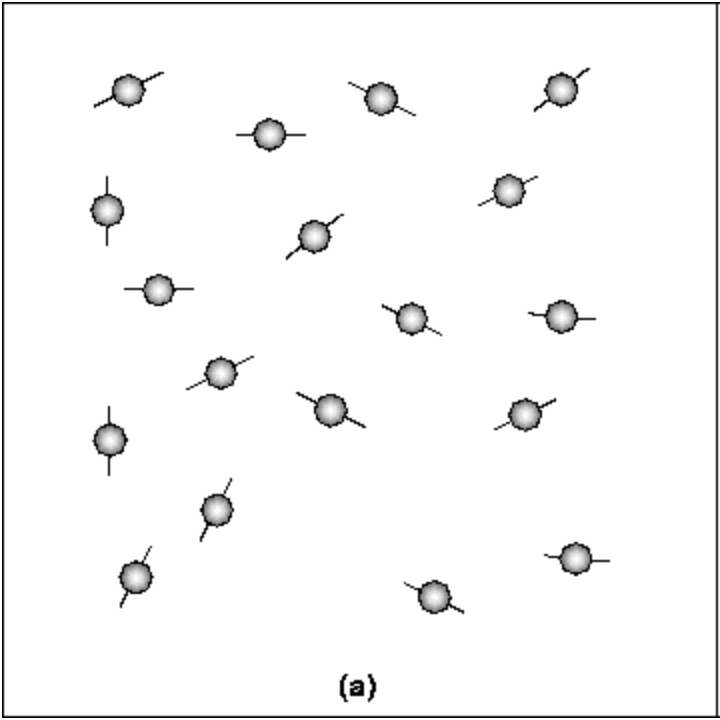
\includegraphics[width=6cm, height=6cm]{media/hydrogen_moving_freely.png}
        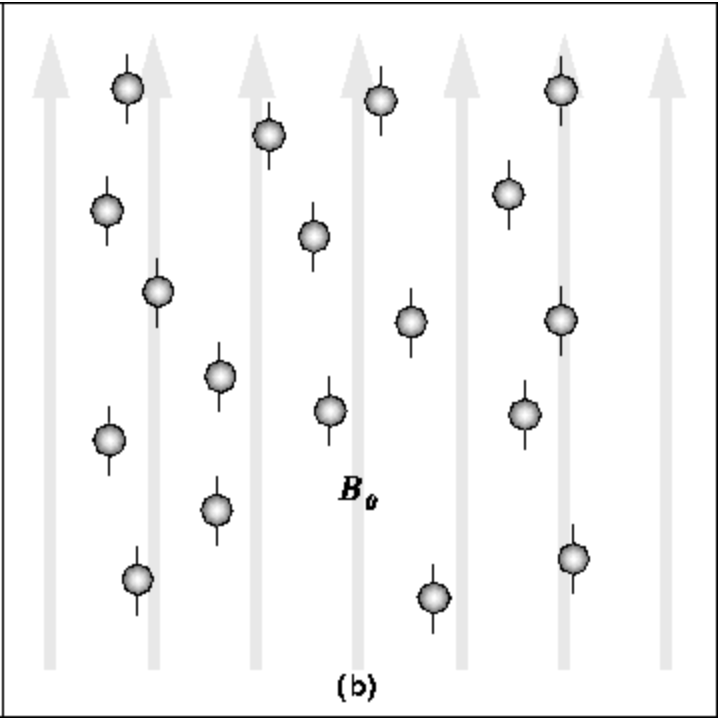
\includegraphics[width=6cm, height=6cm]{media/hydrogen_oscilating.png}
        \captionof{figure}[Voľný pohyb vodíkových jadier a ich zarovnanie v smere $\mathcal{B}_{0}$]{Na ľavom obrázku je možné vidieť voľný pohyb vodíkových jadier a na pravom ich zarovnanie v smere $\mathcal{B}_{0}$ \cite{basic_principles_of_mri}.}
\end {center}

Následne sa aplikuje rádiofrekvenčný impulz $\mathcal{B}_{rf}$ kolmo na $\mathcal{B}_{0}$.
Tento impulz rovnajúci sa frekvencii Larmorovej precesie spôsobí posun $\mathcal{M}$ od $\mathcal{B}_{0}$ \cite{basic_principles_of_mri} (vlastný preklad).

\begin {center}
        \centering
        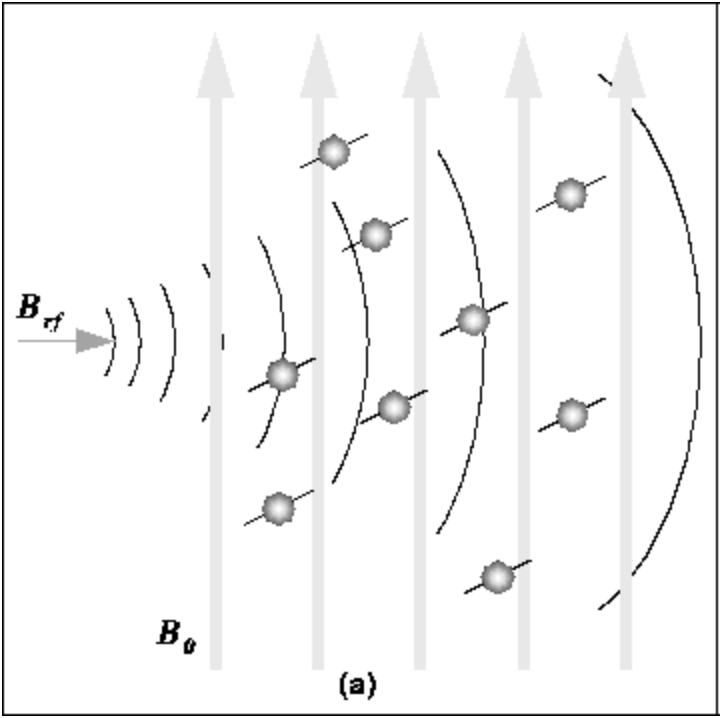
\includegraphics[width=6cm, height=6cm]{media/hydrogen_reacting_to_rf.png}
        \captionof{figure}[Kolmá aplikácia RF impulzu $\mathcal{B}_{rf}$ na vodíkové jadrá]{Kolmá aplikácia RF impulzu $\mathcal{B}_{rf}$ na vodíkové jadrá \cite{basic_principles_of_mri}.}
\end {center}

Frekvenciu Larmorovej precesie (nazývaná ako Larmorova frekvencia), je definovaná nasledovne:

\begin {center}
$\omega_{0}$ = $-\gamma * \mathcal{B}_{0}$,
\end {center}

kde $\gamma$ predstavuje gyromagnetický pomer a $\mathcal{B}_{0}$ intenzitu magnetického poľa.
Gyromagnetický pomer je špecifická konštanta závislá na jadre danej častice. Pre vodík sa táto konštanta rovná 42.6 MHz/Tesla \cite{basic_principles_of_mri} (vlastný preklad). \newline

Akonáhle prestane pôsobiť rádiofrekvenčný impulz $\mathcal{B}_{rf}$, jadrá vodíka sa presunú naspäť tak, že ich $\mathcal{M}$ je znovu paralelný s $\mathcal{B}_{0}$. Tento návrat vodíkových jadier sa nazýva relaxácia. Počas nej jadrá strácajú energiu vysielaním ich vlastného rádiofrekvenčného signálu. Tento signál sa nazýva \uv{voľný indukčný rozpad} -- z anglického Free Induction Decay (FID). Tento signál sa zmeria vodivým poľom MR prístroja za účelom vyhotovenia 3D MR snímku v odtieňoch šedej \cite{basic_principles_of_mri} (vlastný preklad).

\begin {center}
        \centering
        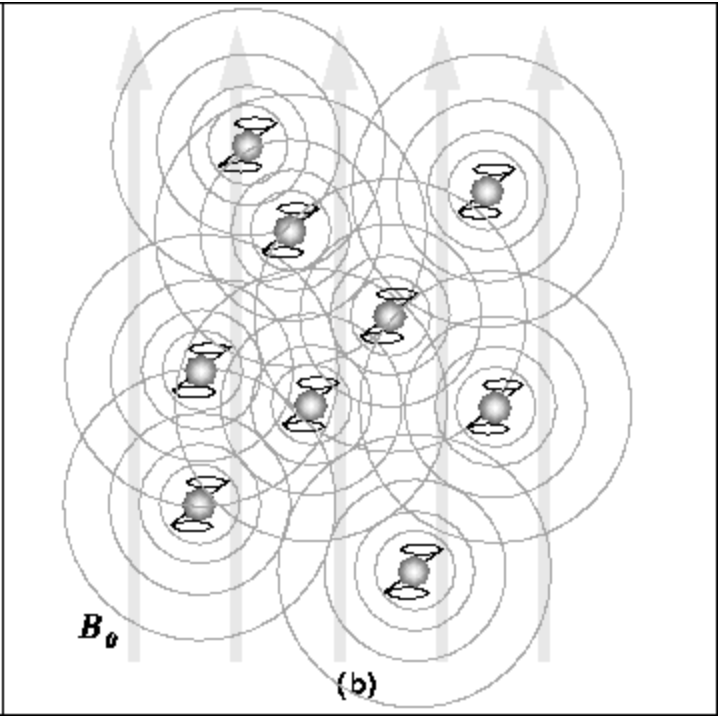
\includegraphics[width=6cm, height=6cm]{media/hydrogen_emitting_rf.png}
        \captionof{figure}[Emitovanie FID signálu vodíkovými jadrami]{Emitovanie FID signálu vodíkovými jadrami \cite{basic_principles_of_mri}.}
\end {center}

Avšak, na jeho vytvorenie musí byť FID signál enkódovaný pre každý rozmer pomocou frekvenčného a fázového kódovania. Kódovanie v axiálnom smere sa dosiahne pridaním gradientového magnetického poľa $\mathcal{G}_{y}$ v smere $\mathcal{B}_{0}$ (v smere $y$). Po pridaní $\mathcal{G}_{y}$ sa hodnota Larmorovej frekvencie zmení lineárne v axiálnom smere, tzn. že pre konkrétny axiálny rez existuje konkrétna Larmorova frekvencia, ktorá sa aplikuje vyslaním rádiofrekvenčného impulzu $\mathcal{B}_{rf}$. $\mathcal{G}_{y}$ sa potom odstráni a ďalší gradient, $\mathcal{G}_{x}$, sa aplikuje kolmo na $\mathcal{G}_{y}$. Výsledkom je, že rezonančné frekvencie jadier sa menia v smere $x$ vďaka $\mathcal{G}_{x}$ a majú fázovú variáciu v smere $y$ v dôsledku predtým aplikovaného $\mathcal{G}_{y}$. Vzorky v smere $x$ sú teda kódované frekvenciou a v smere $y$ fázou. 2D inverzná Fourierova transformácia sa následne použije na transformáciu vzoriek na snímku \cite{basic_principles_of_mri} (vlastný preklad). \newline

Kontrast získanej snímky závisí od nasledujúcich dvoch parametrov:

\begin {itemize}
\item {od času pozdĺžnej relaxácie - T1}
\item {a od času priečnej relaxácie - T2.}
\end {itemize}

Čas T1 je čas potrebný pre jadrá vodíkov k ich relaxácii a čas T2 predstavuje čas potrebný na to, aby sa FID signál prechádzajúci cez dané tkanivo rozpadol. Oba časy závisia od daného typu látky nachádzajúcej sa v subjekte \cite{basic_principles_of_mri} (vlastný preklad).

Po získaní MR snímky sa impulz $\mathcal{B}_{rf}$ opakuje vopred stanovenou rýchlosťou. Zmenou sekvencie impulzov ($\mathcal{B}_{rf}$) sa vytvárajú rôzne typy snímkov. Čas opakovania ($TR$) je množstvo času medzi po sebe nasledujúcimi pulznými sekvenciami aplikovanými na rovnaký rez. Time to Echo ($TE$) je čas medzi dodaním impulzu $\mathcal{B}_{rf}$ a prijatím odozvy. Úpravou $TR$ je možné meniť výsledný kontrast na snímke medzi rôznymi typmi tkanív \cite{basic_principles_of_mri} (vlastný preklad). \clearpage

\section {SPAMM}

SPAMM -- z anglického (SPAtial Modulation of Magnetization) $\rightarrow$ \uv{priestorová modulácia magnetizácie} -- je technika, ktorá používa rádiofrekvenčné saturačné impulzy pre umiestnenie mriežky na myokard, za cieľom sledovania jej pohybu počas srdcového cyklu.

V súčasnej praxi sa SPAMM technika používa v situáciách, kde informácia o kontrakcii myokardu je kľúčová, ako napr. podozrenie na ischemickú chorobu srdca alebo abnormality týkajúcej sa neprirodzeného pohybu steny myokardu \cite{spamm_description} (vlastný preklad).

\begin {center}
        \centering
        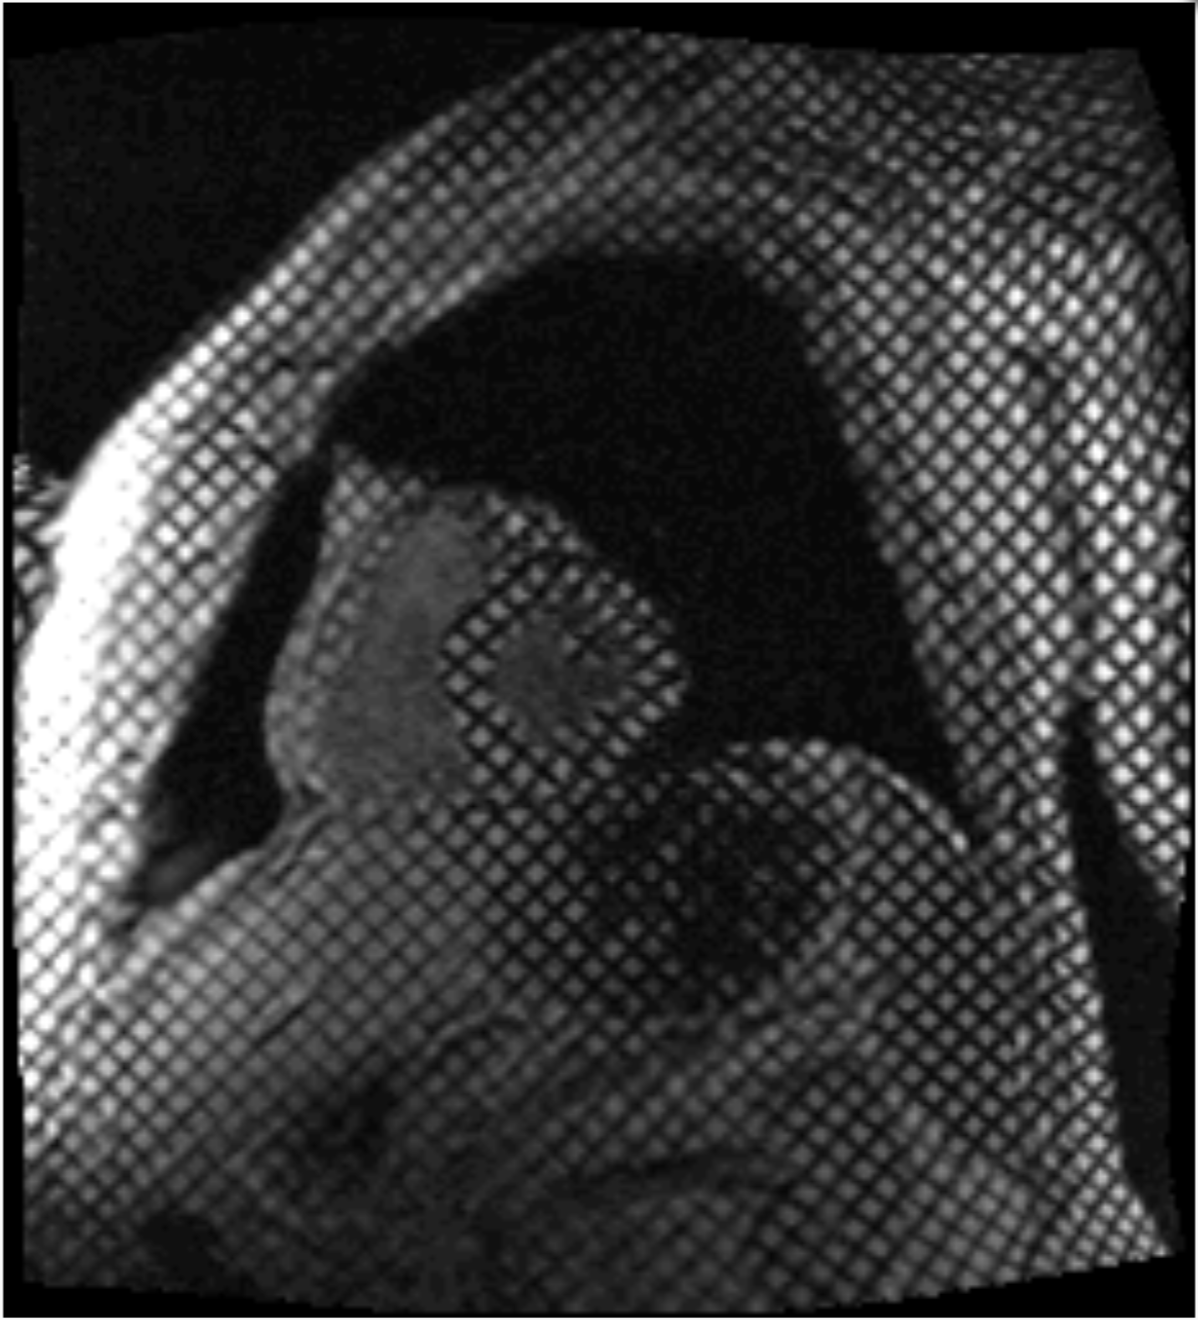
\includegraphics[width=6cm, height=6cm]{media/tagged_heart.png}
        \captionof{figure}[Tagovaný snímok myokardu pomocou techniky SPAMM]{Otagovaný snímok myokardu pomocou techniky SPAMM \cite{spamm_description}.}
\end {center}

Nevýhodou použitia tejto techniky je skutočnosť, že táto mriežka sa stráca s blížiacim sa koncom srdcového cyklu. Samotné čiary mriežky sa pri konci systoly (časť srdcového cyklu, počas ktorej sa komory srdca sťahujú po naplnení krvou) môžu zlúčiť alebo úplne vyblednúť, čo sťažuje následnú analýzu pohybu srdca \cite{spamm_description} (vlastný preklad).

\begin {center}
        \centering
        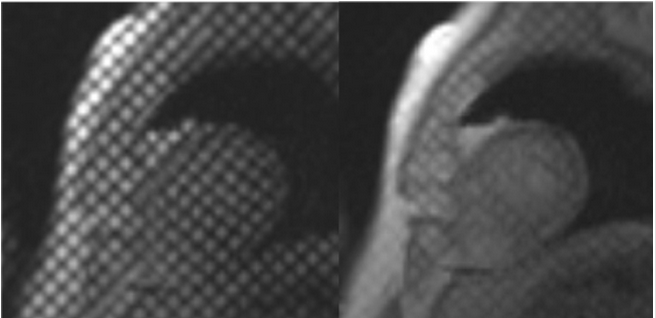
\includegraphics[width=10cm, height=5cm]{media/early_late_systole.png}
        \captionof{figure}[Ukážka vyblednutia SPAMM mriežky]{Ľavý obrázok zobrazuje začiatok systoly, pravý jej koniec.}
\end {center}

\pagebreak

\section {Analýza súčasnej aplikácie}

V tejto sekcii sa budem zaoberať analýzou súčasnej aplikácie, ktorá zahŕňa popis jej funkcionality spolu s vizualizáciami...

\subsection {Popis aplikácie}

Cameo je desktopová aplikácia schopná zobrazovať sériu snímkov myokardu, ktoré pochádzajú z MR. Taktiež zobrazuje doplňujúce údaje, ako napr. údaje o pacientovi, detaily o zobrazených snímkoch a detaily série týchto snímkov. Okrem samotného zobrazenia myokardu aplikácia umožňuje tiež analyzovať myokard. V našom prípade sa analýza myokardu týka jeho pohybu.

Pre analýzu srdcového svalu je potrebné najprv do aplikácie nahrať sériu snímkov, ktoré sú otagované priestorovou moduláciou magnetizácie popísanou vyššie. Táto mriežka sa na každom snímku deformuje podľa pohybu tkaniva. Na počiatočných snímkoch je mriežka dobre viditeľná, avšak jej viditeľnosť sa každým ďalším snímkom zmenšuje. Tento efekt je spôsobený poklesom Nevýhodou  Pohyb myokardu je možný analyzovať vďaka 


Túto aplikáciu môžeme rozdeliť na x častí - potom popíšem každú časť.

\subsection {Použité technológie}

\subsubsection {DICOM}\label{dicom}

V súčasnosti sú snímky získané pomocou zobrazovacích techník v medicíne zväčša ukladané v archivačnom a komunikačnom systéme snímkov. Tento systém ukladá nielen snímkové dáta ale aj iné relevantné dáta k týmto snímkam podľa štandardu známom ako DICOM (Digital Imaging and Communications in Medicine) \cite{Varma_2012} (vlastný preklad). Ten je medzinárodným štandardom pre komunikáciu a manažment informácií o medicínskych obrazových a k nim príslušných dátach. Definuje, ako majú byť takéto dáta spracovávané, ukladané, tlačené a prenášané medzi zariadeniami podporujúcimi príjem týchto dát \cite{about_dicomlibrary} (vlastný preklad).

DICOM štandard bol vyvíjaný na prelome 80. a 90. rokoch 20. storočia v spolupráci medzi American College of Radiology a National Electrical Manufacturers Association \cite{dicom_history} (vlastný preklad). Momentálne sa skladá z 22 nezávislých častí, z ktorých avšak nie všetky musia byť implementované daným zariadením podporujúcim tento štandard.

Pre účely spracovania snímkových dát, DICOM štandard vo svojej 10. časti definuje dátovú štruktúru (formát) súboru, do ktorého sa tieto dáta ukladajú. Dátová štruktúra súboru, ktorý spĺňa podmienky 10. časti tohto štandaru, býva značená ako \uv{DICOM Part 10} súbor, inak známy ako DICOM súbor \cite{Varma_2012} (vlastný preklad).

Štruktúra tohto (binárneho) súboru je nasledovná -- prvých 128 bajtov býva zväčša prázdnych (vyplnených 0). Ďalšie 4 bajty obsahujú uložený reťazec \uv{DICM}.  Na základe týchto bajtov sa dá určiť, či sa jedná alebo nejedná o DICOM súbor.
Ďalej nasleduje hlavička, ktorá je rozdelená na viacero skupín zoskupujúcich súvisiace atribúty. Konkrétne atribúty sa adresujú tagom - ten sa skladá z 8 čísiel v hexadecimálnom formáte. Prvé 4 čísla reprezentujú skupinu, v ktorej sa daný atribút nachádza a posledné 4 čísla jednoznačne identifikujú konkrétny atribút v skupine \cite{Varma_2012} (vlastný preklad).

Ako príklad bude uvedené získanie informácie o pacientovom veku - všetky informácie o pacientovi sa nachádzajú v skupine 0010. Pacientov vek v tejto skupine sa nachádza na pozícii 1010, tým pádom výsledný tag pod ktorým nájdeme vek pacienta je (0010, 1010). Ku každému tagu je jednoznačne priradená reprezentácia jej hodnoty (VR), ktorý určuje dátový typ, formát a dĺžku hodnoty daného atribútu  \cite{Varma_2012} (vlastný preklad).

Po hlavičke nasleduje skupina 7FE0, ktorá už obsahuje dáta o samotných obrazových pixeloch \cite{Varma_2012} (vlastný preklad). Typ kódovania týchto dát určuje Transfer Syntax -- ten udáva, akým spôsobom sú obrazové pixely zakódované. Transfer Syntax obsahuje taktiež informáciu, v akom poradí bajtov sú informácie zakódované (Little Endian vs Big Endian) a aká kompresia obrazových dát bola použitá \cite{dicom_transfer_syntax} (vlastný preklad).

\subsubsection {Qt}

\quad Súčasná aplikácia bola vyvinutá pomocou Qt -- cross-platformového frameworku určeného pre vytváranie aplikácií najmä v jazyku C\texttt{++}. Aplikácie vyvinuté týmto frameworkom majú výhodu v tom, že sú spustiteľné na rôznych operačných systémoch s minimálnym počtom zmien v zdrojovom kóde \cite{qt_description} (vlastný preklad).

Výsadou tohto frameworku je taktiež rozdelenie jeho funkcionality do jednotlivých modulov. Pri následom vytváraní aplikácie sa použijú len také moduly, ktoré sú v danej aplikácii potrebné \cite{qt_description} (vlastný preklad).

V súčasnej aplikácii boli použité nasledovné moduly: 

\begin{itemize}
\item {Qt Core}
\item {Qt Widgets}
\item {Qt GUI}
\item {Qt Test}
\end{itemize}

Qt Core modul obsahuje najpoužívanejšie triedy ako napr. \lstinline{QCoreApplication}, \lstinline{QObject}, \lstinline{QDebug} a iné. Nakoľko sú tieto triedy používané aj inými modulmi, je tento modul implicitne nalinkovaný Qt frameworkom pri budovaní aplikácie \cite{qtcore_description} (vlastný preklad). \newline

Qt Widgets modul poskytuje UI elementy, ktoré sú určené pre vytváranie používateľského rozhrania. Tieto elementy môžu zobrazovať rozličné dáta, prijímať vstup z klávesnice, byť štylizované a zoskupované do rozličných usporiadaní \cite{qtwidgets_description} (vlastný preklad). Existujúca aplikácia používa z modulu napr. triedu \lstinline{QMainWindow}, ktorá je zodpovedná za vykreslenie aplikačného okna a taktiež triedu \lstinline{QGraphicsScene}, ktorá je zodpovedná za vykreslenie obrázkov z magnetickej rezonancie v DICOM formáte. \newline

Qt GUI modul obsahuje triedy určené pre zobrazovanie aplikačného okna a iného grafického obsahu s následnou obsluhou eventov udalostí. Taktiež obsahuje triedy, ktoré sú zodpovedné za zobrazovanie 2D grafiky, fontov a typografie \cite{qtgui_description} (vlastný preklad).
Súčasná aplikácia z tohto modulu používa napr. triedu \lstinline{QImage}, ktorá obsahuje metódy pre priamy prístup k pixelom obrázkov a ich manipuláciu. \newline

Qt Test modul je poskytuje rozličné triedy pre jednotkové testovanie Qt aplikácií a príslušných knižníc \cite{qttest_description} (vlastný preklad) -- v súčasnej aplikácii bol tento modul využitý pri testovaní grafického používateľského rozhrania a funkcionalít súčasnej aplikácie, ako napr. testovanie zmien v nastaveniach vykreslenej mriežky na obrázku z magnetickej rezonancie.

\subsubsection {Qmake}

Pre zjednodušenie písania Makefilov, ktoré definujú, ako má byť program skompilovaný, bol použitý nástroj Qmake. Ten umožňuje vývojárom definovať vytváranie rozličných Makefilov pre daný program pomocou syntaxu definovaného programom Qmake \cite{qmake_description} (vlastný preklad). Výsledkom tohto procesu je súbor s príponou \lstinline{.pro} obsahujúci inštrukcie, ako daný program skompilovať. Následne sa pomocou príkazu \lstinline{qmake} s argumentom cesty k \lstinline{.pro} súboru daný program skompiluje a jeho výsledkom je spustiteľný súbor aplikácie.

\subsubsection {DCMTK}

DCMTK je kolekcia knižníc a aplikácií, ktoré implementujú veľkú časť štandardu DICOM v jazykoch C a C\texttt{++}. Úlohou týchto knižníc je okrem iného skúmanie, vytváranie a konverzia DICOM súborov, manipulácia s pamäťovými médiami a odosielanie a prijímanie obrazových súborov cez internetové pripojenie. Používa sa v nemocniciach a rôznych spoločnostiach po celom svete, kde sa používa ako softvérový základ pri rozličných výskumných projektoch, prototypoch a komerčných produktoch nevynímajúc \cite{dcmtk_description} (vlastný preklad). \newline

V súčasnej aplikácií je DCMTK využitý pre získanie informácií z hlavičiek DICOM súborov, ako napr:

\begin{itemize}
\item {údaje o pacientovi}
\item {údaje o obrazovom súbore}
\item {údaje o sérií obrazových súborov}
\end{itemize}

\subsubsection {TNL}

Template Numerical Library, v skratke TNL, je kolekcia metód, ktoré uľahčujú vývoj efektívnych numerických riešičov. Táto knižnica je implementovaná pomocou C\texttt{++} s cieľom poskytnúť flexibilné a užívateľsky prívetivé rozhranie. TNL poskytuje natívnu podporu pre moderné hardwarové architektúry ako sú viacjadrové CPU, GPU a distribuované systémy, ktoré je možné spravovať cez jednotné rozhranie \cite{tnl_description}.

V súčasnej aplikácii sú z TNL knižnice použité kolekcie ako napr. \lstinline{String} pre manipuláciu s reťazcami a \lstinline{Containers::Array}, \lstinline|Containers::{Vector,StaticVector,MultiVector}|, čo sú kontajnery reprezentujúce n-dimenzionálne polia, ktoré abstrahujú manažment dát a exekúciu bežných operácií na rozličných hardvérových architektúrach.

Aplikácia z TNL knižnice taktiež používa \lstinline{Solvers::ODE::Merson} -- jedná sa o Runge-Kutta-Merson metódu štvrtého rádu s adaptívnym výberom časového kroku, pomocou ktorej vieme získať približné riešenie diferenciálnych rovníc.

\subsection {Pomocné podprogramy}



\section {Analýza webovej aplikácie}

\subsection {Analýza požiadaviek}

\subsubsection {Funkčné požiadavky}

\subsubsection {Nefunkčné požiadavky}

\subsection {Používateľské role}

\subsection {Prípady použitia}

\chapter {Návrh aplikácie}

\section {Návrh architektúry webovej aplikácie}

\subsection {Client-server vs WebAssembly}

\subsection {Voľba architektúry webovej aplikácie}

\section {Voľba technológií}

\subsection {Technológie pre vývoj webovej aplikácie}

\subsubsection {Frontend}

\subsubsection {Backend}

\subsubsection {Spracovanie DICOM dát}

\subsubsection {Vykreslenie a manipulácia s interaktívnou mriežkou}

\subsection {Prepojenie webového rozhrania s podprogramom}

\section {Návrh používateľského rozhrania}

\section {Komunikácia medzi serverom a klientom}

\subsection {Anonymizácia DICOM dát}

\chapter {Implementácia}

\section {Frontend}

\subsection {Používateľské rozhranie}

\subsection {Spracovanie DICOM dát}

\subsection {Interaktívna úprava mriežky}

\section {Backend}

\subsection {Výpočet umiestnenia mriežky}

\chapter {Testovanie}
Testovanie je neoddeliteľnou súčasťou vývojového procesu aplikácie. To isté platí pre vyvinutú webovú aplikáciu v rámci tejto diplomovej práce.

Po dokončení jej implementácie bola aplikácia zverená trom testerom -- Erikovi Ekeovi, Timei Bartalskej a ZZZ. ZZZ je odborníkom na magnetickú rezonanciu, ktorého momentálne pracovisko je Institut klinické a experimentální medicíny (IKEM) v Prahe. \todo {doplniť meno testera z IKEMU sem a do poďakovania}

\section {Zoznam zaznamenaných problémov aplikácie}
Testovanie aplikácie prebehlo podľa scenárov všetkých prípadov použitia. Výsledkom testovania webovej aplikáce boli nasledujúce pripomienky:
\begin {itemize}
\item {nefunguje nastavenie rýchlosti animácie počas animácie snímok,}
\item {zoomovanie alebo odzoomovanie snímky nie je možné v niektorých prípadoch zastaviť,}
\item {neočakávané správanie polí pre zadávanie $x$ a $y$ offsetov mriežky,}
\item {nemožnosť opustiť aktivovaný nástroj pre pohyb snímky,}
\item {nemožnosť scrollovania pre zmenu indexu zobrazenej snímky a}
\item {absencia automatického zapnutia nástroja pre pohyb s mriežkou pri zmene jej módu}
\end {itemize}

Tieto pripomienky boli do webovej aplikácie riadne zapracované a verifikované samotnými testermi.
Príčiny týchto problémov je možné nájsť v nasledujúcej sekcii.

\section {Popis príčin zaznamenaných problémov}
Nefunkčné nastavenie rýchlosti bolo spôsobené nefungujúcou detekciou pohybu slidera určenom pre zmenu rýchlosti animácie snímok počas ich animácie. Táto situácia bola ošetrená detekciou tejto situácie.

Čo sa týka problému zoomovania, resp. odzoomovania snímiek, daný problém spočíval v situácii, kedy sa \texttt{mouseup}\footnote{https://developer.mozilla.org/en-US/docs/Web/API/Element/mouseup\textunderscore event} event emituje mimo ikony určenej pre zoomovanie/odzoomovanie snímky. Tento problém bol ošetrený pridaním \texttt{mouseup} event listeneru v rámci celého dokumentu, ktorý sa aktivoval počas zoomovania, resp. odzoomovania snímky.

Neočakávané správanie polí pre $x$ a $y$ offsety bol spôsobený ich skracovaním na dve desatinné miesta, čo viedlo k zadaniu iných čísiel aké boli zadávané. Odstránenie tejto modifikácie odstránil ohlásený problém.

Situácia, ktorá neumožňovala opustiť nástroj pre pohyb snímky nastala, ak bol aktivovaný tento nástroj pred vymazaním používateľom vygenerovanej mriežky, keďže aplikácia v prípade neexistencie mriežky neumožňovala prepnúť na tlačidlo pohybu s mriežkou. Tento problém bol vyriešený pridaním možnosti vypnutia daného nástroja pomocou opätovného kliknutia na daný nástroj.

Nemožnosť zmeniť zobrazenú snímku pomocou skrolovania myšou nebolo samo o sebe chybou, avšak iba chýbajúcou vlastnosťou. Avšak túto vlastnosť implementujú aj iné aplikácie, ktoré pracujú so snímkami z magnetickej rezonancie. Dôsledkom toho bola táto vlastnosť implementovaná pomocou využitia \texttt{StackScrollWheel} nástroja z Cornerstone Tools knižnice. Tento nástroj je aktivovaný automaticky pri spustení webovej aplikácie.

\clearpage

Absencia automatického zapnutia nástroja pre pohyb s mriežkou alebo jej bodmi pri zmene jej módu zhoršovalo UX používateľa s aplikáciou, nakoľko je možné očakávať, že pri zmene módu tohto nástroja chce následne používateľ s týmto nástrojom pracovať. Tento chýbajúci krok bol implementovaný automatickým aktivovaním daného nástroja v prípade detekcie zmeny jeho módu.

\appendix\appendixinit % do not remove these two commands

\chapter{Nějaká příloha}


Sem přijde to, co nepatří do hlavní části.
 % include `appendix.tex' from `text/' subdirectory

\backmatter % do not remove this command

\printbibliography % print out the BibLaTeX-generated bibliography list

\chapter{Obsah priloženého .zip súboru}

\begin{figure}
	\dirtree {%
		.1 diploma-thesis\DTcomment{adresár so zdrojovými kódmi}.
		.2 app\DTcomment{adresár so zdrojovými kódmi aplikácie}.
		.2 thesis\DTcomment{adresár so zdrojovým kódom práce vo formáte \LaTeX{}}.
		.3 DP\_Tomáš\_Taro\_2023.pdf\DTcomment{text práce vo formáte PDF}.
	}
\end{figure}

\end{document} % include `medium.tex' from `text/' subdirectory

\end{document}
